\documentclass{beamer}
\usepackage[utf8]{inputenc}
\usepackage{amsmath, pdfpages, pdflscape, lscape, color, listings, hyperref, amssymb, graphicx,textcomp,varioref, afterpage, subcaption, float, bm, tikz, multicol} 

\global
\newcommand{\Fig}[1]{Figure \ref{#1}}
\newcommand{\fig}[1]{figure \ref{#1}}
\newcommand{\tab}[1]{table \ref{#1}}
\newcommand{\eq}[1]{equation \ref{#1}}
\newcommand{\Eq}[1]{Equation \ref{#1}}
\newcommand{\alg}[1]{algorithm \ref{#1}}
\newcommand{\Alg}[1]{Algorithm \ref{#1}}
\newcommand{\chp}[1]{chapter  \ref{#1}}
\newcommand{\Chp}[1]{Chapter  \ref{#1}}
\newcommand{\e}[1]{\cdot 10^{#1}}
\newcommand{\h}{\hbar}
\newcommand{\der}[2]{\frac{\partial #1}{\partial #2}}
\newcommand{\dder}[2]{\frac{\partial^2 #1}{\partial #2^2}}
\newcommand{\p}{\boldsymbol{P}}
\newcommand{\q}{\boldsymbol{q}}
\newcommand{\norm}[1]{\left\lVert#1\right\rVert}
\newcommand{\coef}[2]{\frac{\langle #1,#2\rangle_Q}{\norm{#2}^}}


\newenvironment{test}[1]
{
 \usebackgroundtemplate{}
 \color{gray!30!black}
   \begin{tikzpicture}[remember picture, overlay]
     \node[anchor = center, opacity=.25] (image) at (current page.center) {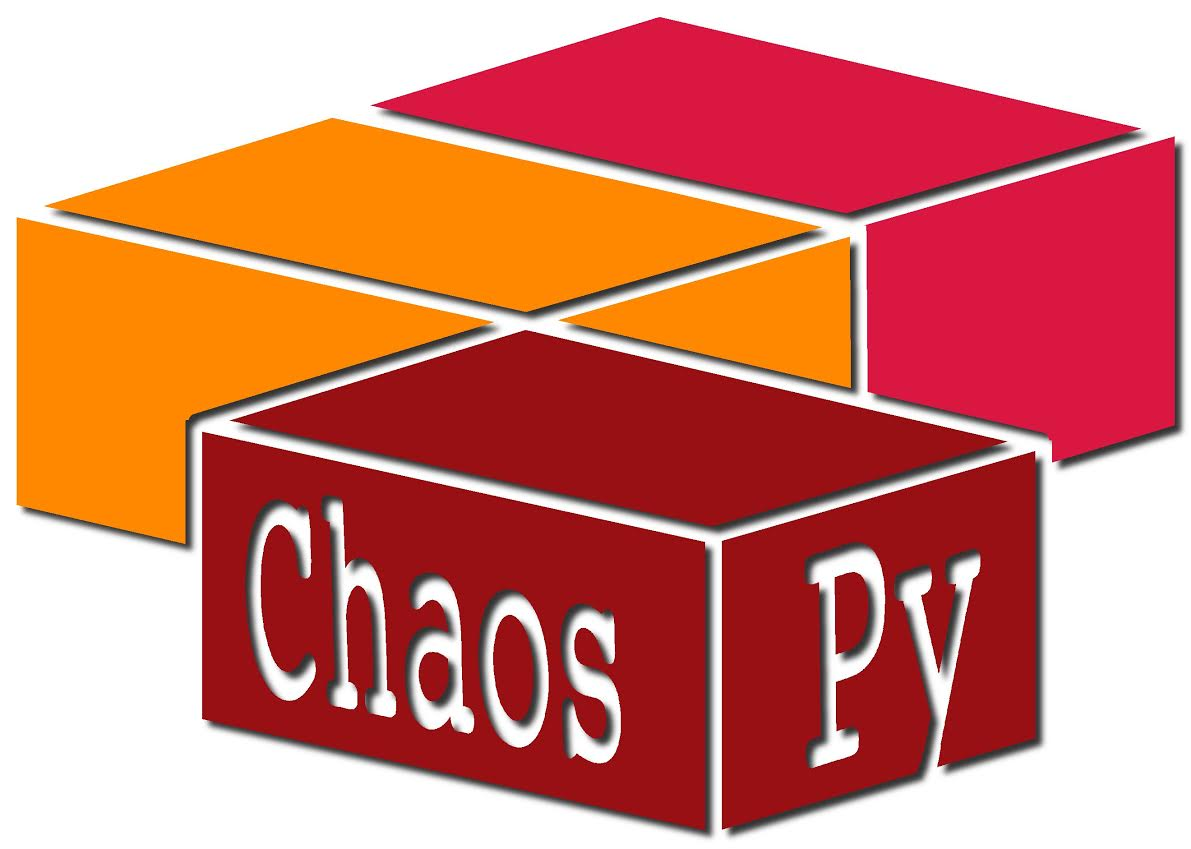
\includegraphics[scale=0.25]{chaospy_logo.jpg}};
   \end{tikzpicture}
 \begin{frame}[fragile,enviroment=chaospy]
   
}
{
 \end{frame}
}

\lstset{
escapeinside=||
}


\newenvironment{chaospy}[1]
{\color{gray!30!black}
     \color{gray!30!black}
     \usebackgroundtemplate{
   \begin{tikzpicture}[remember picture, overlay]
     \node[anchor = center, opacity=.25] (image) at (current page.center) {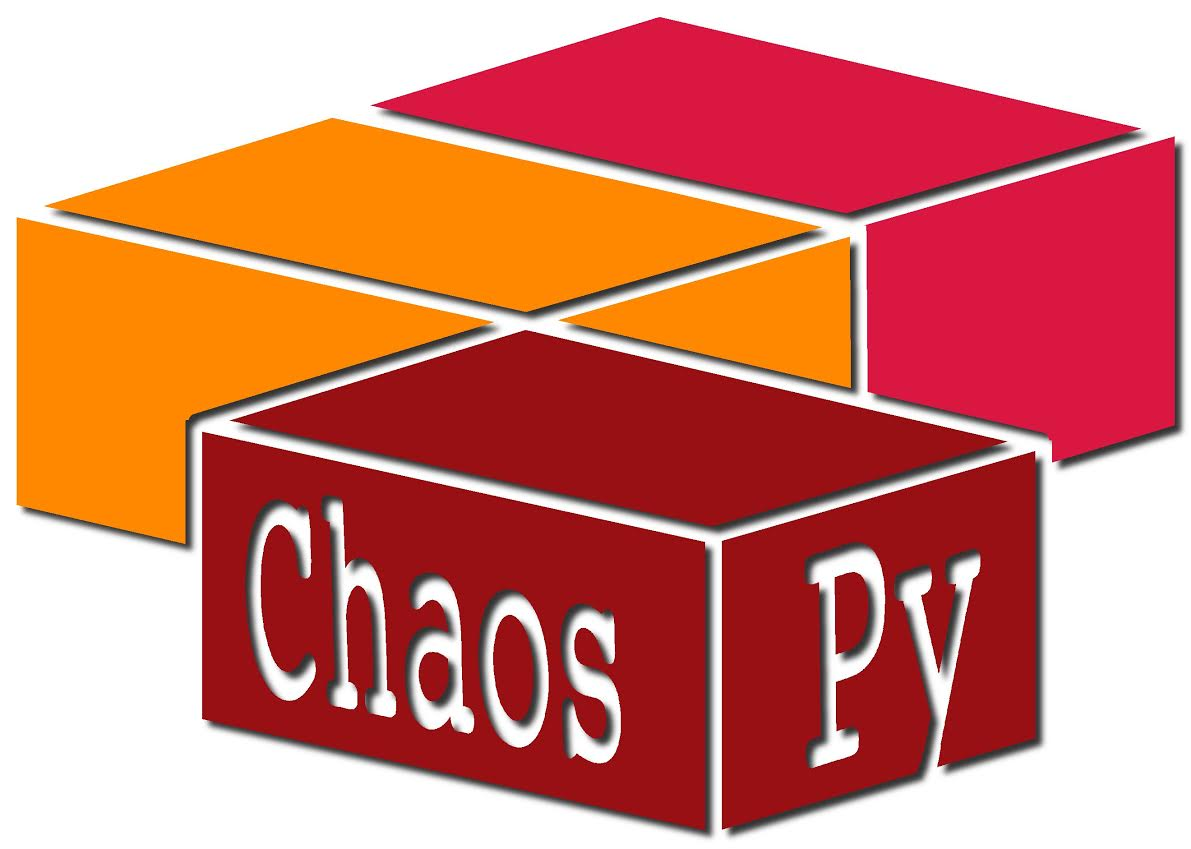
\includegraphics[scale=0.25]{chaospy_logo.jpg}};
   \end{tikzpicture}}
     \begin{frame}[fragile,environment=chaospy]
    \frametitle{{#1}}}
{\end{frame}}


\definecolor{keywords}{RGB}{255,0,90}
\definecolor{comments}{RGB}{0,0,113}
\definecolor{red}{RGB}{160,0,0}
\definecolor{green}{RGB}{0,150,0}
 
\usetheme{kalkulo}

\graphicspath{{./figures/}}


\title{Polynomial chaos expansions part 3: Advanced topics - Intrusive gallerkin method}
\author{Jonathan Feinberg and Simen Tennøe}


\begin{document}



\begin{frame}
  \maketitle
\end{frame}

\begin{frame}
 \frametitle{Repetition: The problem}
  We have a simple differential equation
  \begin{align*}
    \frac{d u(x)}{dx} & =-au(x),\qquad u(0) = I,
  \end{align*}
  \pause
  With the solution:
  \[u(x) = Ie^{-a(x)}\]
  \pause
  where
   \[a \sim \text{Uniform(0, 0.1)}, \qquad I \sim \text{Uniform(8, 10)}\] 
   \pause
   And we approximate it with
   \[u \approx \hat u_M = \sum_{n=0}^Nc_nP_n\]
\end{frame}

\begin{frame}
 \frametitle{Intrusive gallerkin method, initial condition}
 \begin{align*}
 \hat u_M(0) &= I\\
  \onslide<2-> {\sum_{n=0}^Nc_n(0)P_n &= I}\\
  \onslide<3-> {\langle\sum_{n=0}^Nc_n(0)P_n,P_k\rangle &= \langle I,P_k\rangle }\\
  \onslide<4-> {\sum_{n=0}^Nc_n(0)\langle P_n,P_k\rangle &= \langle I,P_k\rangle }\\
  \onslide<5-> {\sum_{n=0}^Nc_n(0)E(P_nP_k) &= E(IP_k)}\\
   \onslide<6-> {c_n(0) &= \frac{E(IP_k)}{E(P_n^2)}}\\
   \end{align*}

\end{frame}


\begin{frame}
 \frametitle{Intrusive gallerkin method}
 \begin{align*}
  \frac{d}{dx}\left(\hat u_M \right) &= -a \hat u_M\\
  \onslide<2-> {\frac{d}{dx}\left(\sum_{n=0}^Nc_nP_n \right) &= -a \sum_{n=0}^Nc_nP_n}\\
 \onslide<3-> {\langle \frac{d}{dx}\left(\sum_{n=0}^Nc_nP_n \right),P_k\rangle &= \langle-a \sum_{n=0}^Nc_nP_n,P_k\rangle}\\
 \onslide<4-> {\frac{d}{dx}\sum_{n=0}^Nc_n\langle P_n ,P_k\rangle &= -\sum_{n=0}^Nc_n\langle aP_n,P_k\rangle}\\
 \onslide<5-> {\frac{d}{dx}\sum_{n=0}^Nc_n E(P_nP_k)&= -\sum_{n=0}^Nc_n E(aP_nP_k)}\\
 \end{align*}

 
\end{frame}



\begin{frame}
 \frametitle{Intrusive gallerkin method}
 \begin{align*}
 \frac{d}{dx}c_n &= -\frac{E(aP_nP_k)}{E(P_n^2)}c_n\\
 c_n(0) &= \frac{E(IP_k)}{E(P_n^2)}
 \end{align*}
 This is a differential equation for $c_n$ that we can solve.

 \end{frame}

 
\begin{frame}
 \frametitle{We now have two expectation values to calculate, $E(P_nP_k)$}
% \[E(P_nP_k) = E \left(\left[\begin{matrix}
%                P_0^2 &0&0&0&0&0 \\
%                0& P_1^2 &0&0&0&0\\
%                0&0& P_2^2 &0&0&0\\
%                0&0&0& P_3^2 &0&0\\
% 	       0&0&0&0& P_4^2 &0\\
%                0&0&0&0&0& P_5^2\\
%                \end{matrix}\right]\right)
% \]
   \begin{figure}
  %\caption{Binary matrix of $E(aP_nP_k)$}
  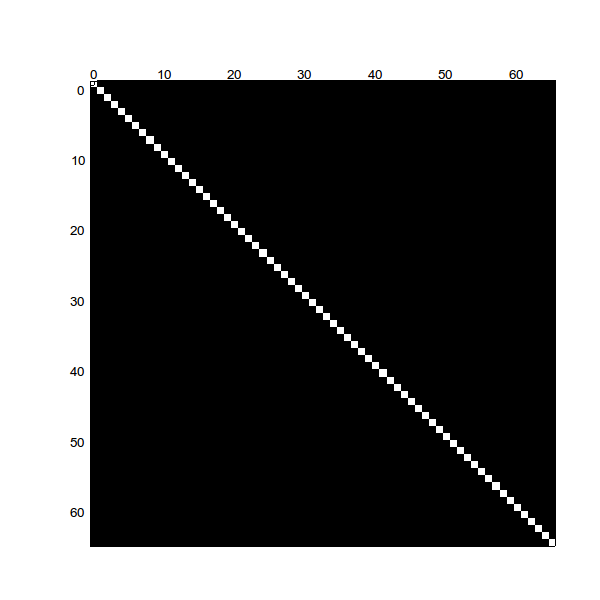
\includegraphics[width=0.65\textwidth]{binary_matrix1.png}
 \end{figure}
 \end{frame}


\begin{frame}
 \frametitle{We now have two expectation values to calculate, $E(aP_nP_k)$}
  \begin{figure}
  %\caption{Binary matrix of $E(aP_nP_k)$}
  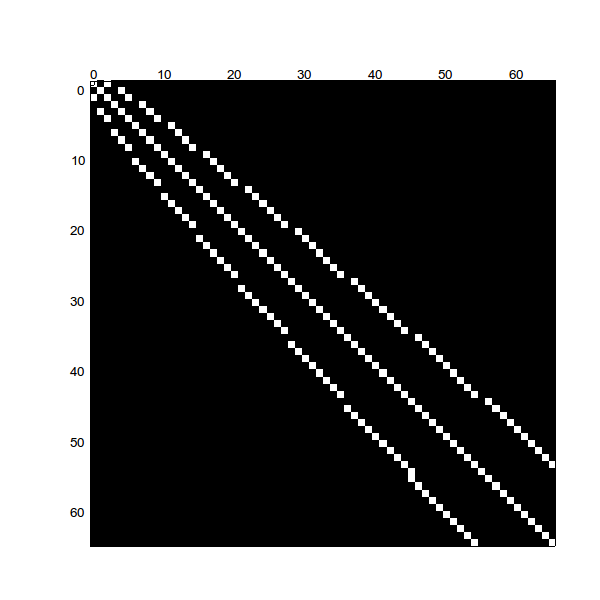
\includegraphics[width=0.65\textwidth]{binary_matrix.png}
 \end{figure}
 \end{frame}

 
 \begin{chaospy}{}
    \scriptsize
\begin{lstlisting}[language=python]
n = 2
P = cp.orth_ttr(n, dist)

N = len(P)
q0, q1 = cp.variable(2)

P_nn = cp.outer(P, P)
E_ank = cp.E(q0*P_nn, dist)
E_nn = cp.E(P_nn, dist)
E_ik = cp.E(q1*P, dist)

def f(c_n,x):
    return -c_n/E_nn*np.sum(E_ank,0)

solver = odespy.RK4(f)

c_0 = sum(E_ik,0)/E_nn
print c_0
solver.set_initial_condition(c_0)
c_n, x_ = solver.solve(x)
\end{lstlisting}
\end{chaospy}


\begin{frame}
 \frametitle{Convergence of gallerkin method}
  \begin{figure}
  %\caption{Binary matrix of $E(aP_nP_k)$}
  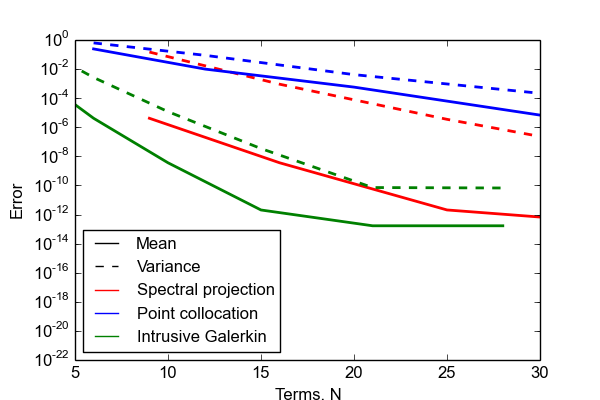
\includegraphics[width=0.65\textwidth]{convergence_gallerkin.png}
 \end{figure}
\end{frame}












\end{document}
